%! TEX root = main.tex
This section shows cases for V\&V (verification and validation).
PetIBM is a baseline in PINNs benchmarks, so its correctness must be confirmed.
The cases shown here include 2D and 3D Taylor-Green vortex, 2D cylinder flows, 3D flow around a sphere, and 3D flow around an inclined flat plate.

\subsection*{Convergence test of 2D Taylor-Green vortex at $Re=100$}

The Taylor-Green vortex (TGV) represents a family of flows with a specific form of analytical initial flow conditions in 2D and 3D.
Specifically, 2D TGV problems with periodic boundary conditions have closed-form analytical solutions; hence, they usually serve as standard verification cases for CFD solvers. 
Here we used the following 2D Taylor-Green vortex to examine the order of convergence:
\begin{equation}\label{eq:tgv}
    \left\{
        \begin{aligned}
            u(x, y, t) &= V_0\cos(\frac{x}{L})\sin(\frac{y}{L})\exp(-2\frac{\nu}{L^2}t) \\
            v(x, y, t) &= - V_0 \sin(\frac{x}{L})\cos(\frac{y}{L})\exp(-2\frac{\nu}{L^2}t) \\
            p(x, y, t) &= -\frac{\rho}{4}V_0^2\left(cos(\frac{2x}{L}) + cos(\frac{2y}{L})\right)\exp(-4\frac{\nu}{L^2}t)
        \end{aligned}
    \right.
\end{equation}
$V_0$ represents the peak (and lowest) velocity at $t=0$;
$L$ is a scaling factor in the spatial domain;
$\nu$ and $\rho$ are kinematic viscosity and density, respectively.
$u$ and $v$ denote the velocity components in the $x$ and $y$ directions.
$p$ is the pressure.
The periodic boundary conditions are applied to $x=-L\pi$, $x=L\pi$, $y=-L\pi$, and $y=L\pi$.
As shown in the analytical solutions, the flow patterns do not change spatially, and only the amplitudes decay exponentially in time.

We used the following parameters for all our computational experiments: $V_0=L=\rho=1.0$ and $\nu=0.01$.
These parameters correspond to a Reynolds number of $Re=100$.

As the TGV problem only has periodic boundary conditions, there is no boundary discretization error in PetIBM that will taint the overall spatial convergence.
A 2nd-order grid convergence in space should therefore be expected.
The time marching schemes are Adams-Bashforth for the convection and Crank-Nicolson for the diffusion, so a 2nd-order convergence in time should also be observed.
Overall, the spatial-temporal convergence should be the 2nd-order.
Hence, we conducted a convergence test on spatial-temporal space for  convenience and simplicity.
The $L_2$ spatial-temporal error in this work is defined as:
\begin{equation}\label{eq:spt-err-def}
    \begin{aligned}
    L_{2,sp-t} \equiv &\sqrt{
        \frac{1}{L_x L_y T}
        \int\limits_{x} \int\limits_{y} \int\limits_{t} \lVert f - f_{ref} \rVert^2 \diff x \diff y \diff t
    } \\
    = &
    \sqrt{\frac{1}{N_x N_y N_t}\sum\limits_{i=1}^{N_x}\sum\limits_{j=1}^{N_y}\sum\limits_{k=1}^{N_t}\left(f^{(i, j, k)} - f_{ref}^{(i, j, l)}\right)^2}
    \end{aligned}
\end{equation}
$N_x$, $N_y$, and $N_t$ represent the number of cells on the $x$, $y$, and $t$ axis.
$f$ is the flow quantity of our interest, and $f_{ref}$ is the corresponding analytical solution.
The superscript $(i, j, k)$ denotes the value at the $(i, j, k)$ point in the discretized spatial-temporal space.
The characteristic cell size in a spatial-temporal sense is simply $\sqrt[3]{\frac{1}{N_x N_y N_t}}$, meaning the characteristic number of cells is $\sqrt[3]{N_x N_y N_t}$.

We ran simulations with $2^{n} \times 2^{n}$ cells for $i=4, 5, \dots, 10$.
The simulations ran from $t=0$ up to $t=100$, and we output the transient results every $2$ seconds of $t$.
The time step size $\Delta t$ did not follow a fixed refinement ratio.
Rather, it was refined based on the maximum allowed CFL number and whether it was a factor of $2$ (to output transient results).
The corresponding time step sizes were $\Delta t = 1.25e-1, 8e-2, 4e-2, 2e-2, 1e-2, 5e-3, 1.25e-3$.
The linear solvers for both velocity and pressure systems were solved with BiCGSTAB (biconjugate gradient stabilized method).
The velocity and pressure systems used a block Jacobi preconditioner and an algebraic multigrid preconditioner from AmgX.
At each time step, both solvers stopped when preconditioned residual reached $1e-14$.
The hardware contains 5 physical cores of Intel E5-2698 v4 and 1 V100 GPU.

Figure \ref{fig:petibm-tgv2d-re100-conv} shows the grid convergence results.
\begin{figure}[hbt!]
    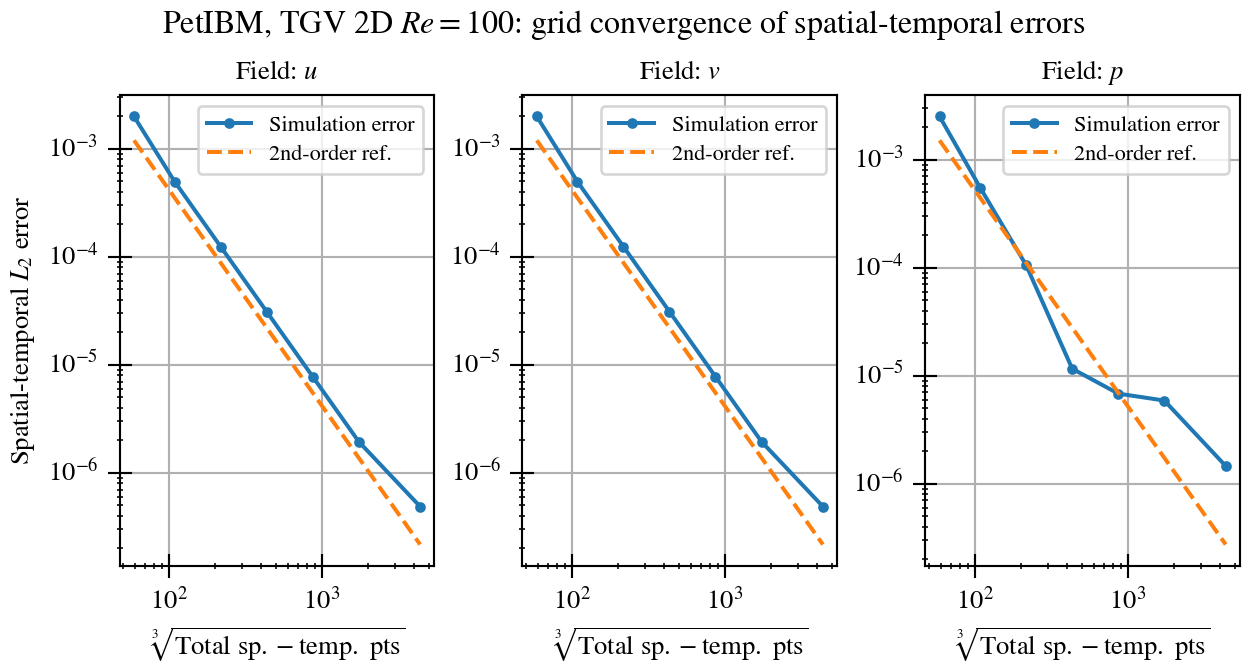
\includegraphics[width=0.75\linewidth]{tgv-2d-re100/petibm-tgv-2d-re100-convergence}
    \caption{PetIBM, 2D TGV, $Re=100$: spatial-temporal grid convergence}
    \label{fig:petibm-tgv2d-re100-conv}
\end{figure}
Both $u$ and $v$ velocities follow an expected 2nd-order convergence before machine truncation errors become non-trivial at the $1024 \times 1024$ grid.
However, the pressure field does not follow such a nice convergence pattern.
After examining the log files, we determined that the cause was that AmgX did not solve the pressure systems to the tolerance we defined.
AmgX has a hard-coded stop mechanism when relative residuals (relative to the residual before the 1st iteration in a Krylov solver) reach the machine precision.
So while we configured the tolerance to be $1e-14$, the final preconditioned residuals of the pressure systems did not match this value.
On the other hand, the velocity systems were solved to the requested tolerance.

As we determined that the cause of the deviated convergence in pressure was irrelevant to the numerical method implementation, we concluded that the 2D TGV verification was successful.

\subsection*{Verification of 3D Taylor-Green vortex at $Re=1600$}

3D TGV problems have closed-form initial conditions but do not have closed-form analytical solutions.
These 3D TGV problems differ from 2D TGV cases due to the transition to turbulence.
Hence, it serves as a standard benchmark for turbulence simulations.
For example, see the campaign described in \cite{noauthor_1st_2012}. 
We compared the results to the other published simulation data \cite{debonis_solutions_2013} in this verification.

The initial condition used was
\begin{equation}\label{eq:tgv3d-ic}
    \left\{
    \begin{aligned}
        u &=V_{0} \sin \left(\frac{x}{L}\right) \cos \left(\frac{y}{L}\right) \cos \left(\frac{z}{L}\right) \\
        v &=-V_{0} \cos \left(\frac{x}{L}\right) \sin \left(\frac{y}{L}\right) \cos \left(\frac{z}{L}\right) \\
        w &=0 \\
        p &=\frac{\rho V_{0}^{2}}{16}\left(\cos \left(\frac{2 x}{L}\right)+\cos \left(\frac{2 y}{L}\right)\right)\left(\cos \left(\frac{2 z}{L}\right)+2\right)
    \end{aligned}
    \right.
\end{equation}
We used $\rho = V_0 = L = 1$ and $\nu=0.000625$, corresponding to $Re \equiv \frac{V_0 L}{\nu} = 1600$.
The computational domain is $-L\pi$ to $L\pi$ for all three directions.

Due to the hardware required for high-resolution 3D DNS simulations for turbulence flow, we did not run the simulation with the spatial resolution suggested by \cite{noauthor_1st_2012}.
Our spatial resolution was $N_x=N_y=N_z=256$ with $\Delta t=0.01$.
The simulation ran up to $t=20$.
The hardware used was 128 physical CPU cores of AMD EPYC 7742 and 4 A100 GPUs (the 80GB variant).
It required about 250GB of memory, and the run time was 37 minutes.

Figure \ref{fig:petibm-tgv3d-re1600-val} shows that the mean kinetic energy qualitatively matches the reference data in \cite{noauthor_1st_2012} and \cite{debonis_solutions_2013}.
\begin{figure}[hbt!]
    \centering
    \begin{subfigure}[b]{0.45\textwidth}
        \centering
        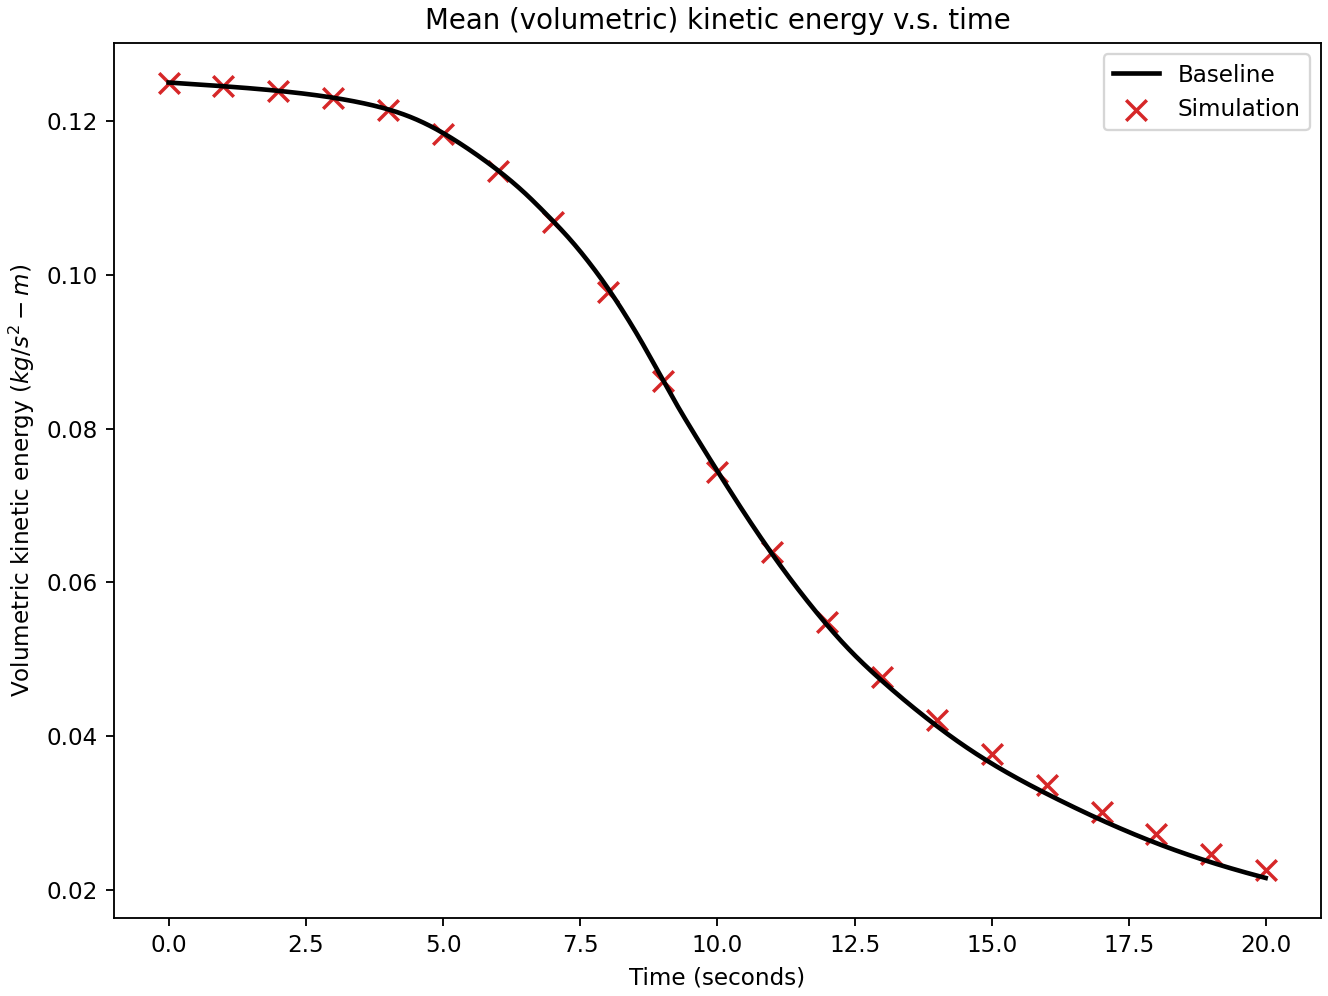
\includegraphics[width=\textwidth]{tgv-3d-re1600/mean-kinetic-energy}
        \caption{Mean kinetic energy}
        \label{fig:petibm-tgv3d-re1600-mean-energy}
    \end{subfigure}
    \hfill
    \begin{subfigure}[b]{0.45\textwidth}
        \centering
        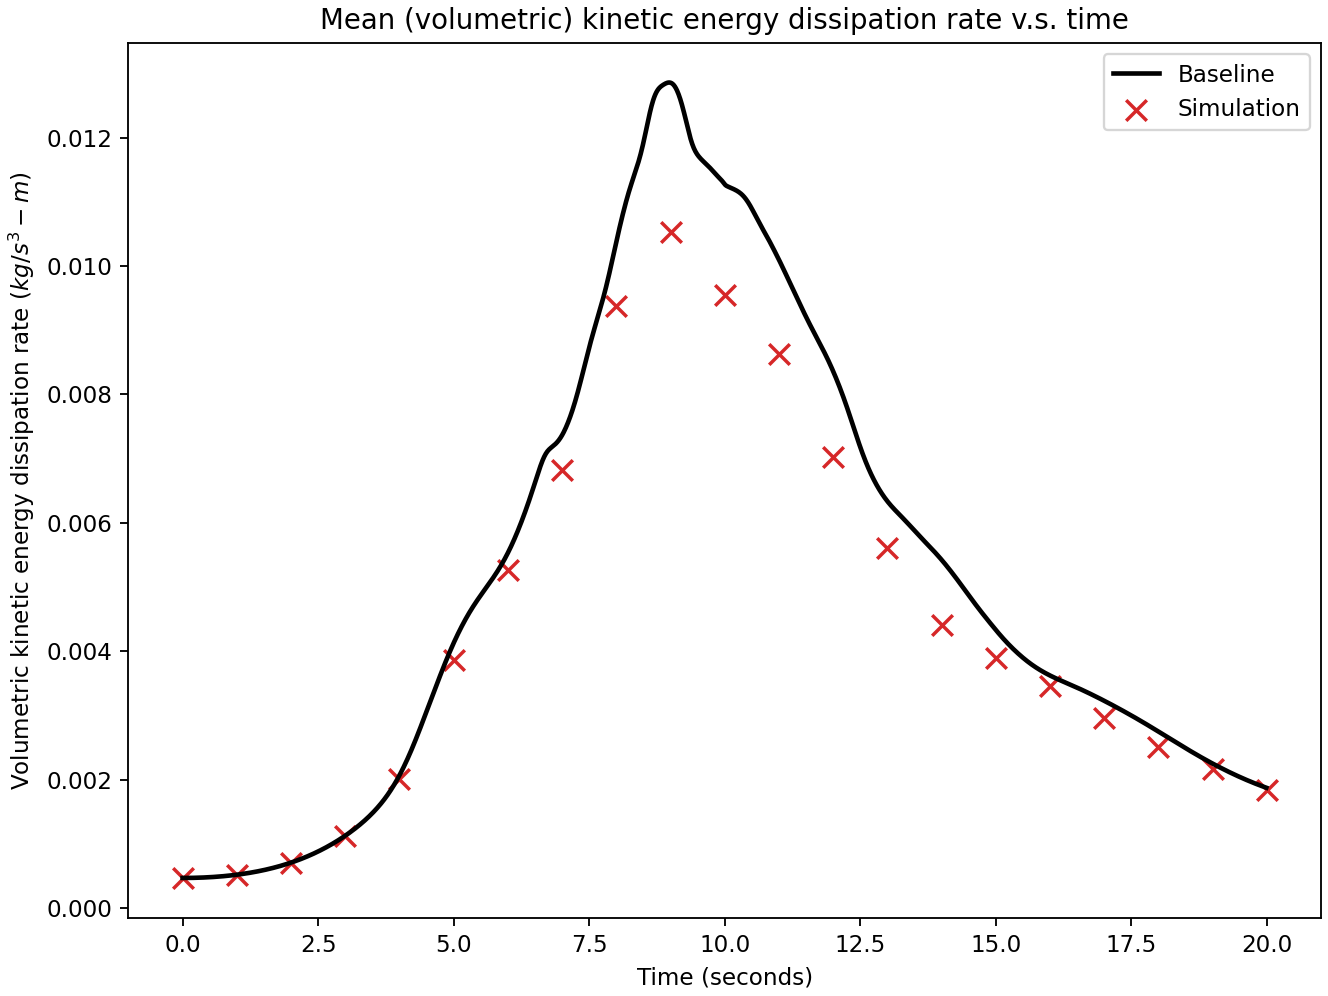
\includegraphics[width=\textwidth]{tgv-3d-re1600/mean-kinetic-energy-dissipation-rate}
        \caption{Mean kinetic energy dissipation rate}
        \label{fig:petibm-tgv3d-re1600-mean-energy-dissp}
    \end{subfigure}
    \caption{PetIBM, 3D TGV, $Re=1600$: validations}
    \label{fig:petibm-tgv3d-re1600-val}
\end{figure}
However, a visible mismatch exists in the mean kinetic energy dissipation rate.
Besides lower spatial resolution, another likely source of error may be in the post-processing rather than in the numerical method implementation.
We calculated the dissipation rate using enstrophy, which requires post-processing steps due to using a staggered grid.
First, we applied the curl operator to the velocity defined on the staggered grid, and the resulting vorticity was also distributed staggered.
Next, we applied the linear interpolation operator and collected values from staggered grid points to cell centers.
Finally, we integrated the cell-centered vorticity using a simple 1st-order numerical integration.
Hence, we suspected that the post-processing largely contributed to the energy dissipation rate error.

Even some results from the campaign of \cite{noauthor_1st_2012} and \cite{debonis_solutions_2013} show this level of mismatch in the dissipation rate.
Therefore, we conclude the 3D TGV verification at this point.
We do not claim that PetIBM's results match the reference data.
Nevertheless, it does not show any concerning problems in the comparison, either.

\subsection*{Validation and verification of 2D Cylinder flows}

In this work, a total of three different 2D cylinder flows were simulated: $Re=40$, $Re=100$, and $Re=200$.
In Williamson's stability categorization \cite{williamson_vortex_1996}, they correspond to the stable, 2D instability, and 2D to 3D transitioning regimes.
The cases of $Re=40$ and $Re=200$ were used for benchmarking PINNs.
Their results and V\&V can be found in chapter \ref{chap:pinn-cases}.
In this section, we only verify and validate our numerical solutions with $Re=100$ only.

The computational domain was $[-15, 35]\times[-25, 25]$ with a spatial discretization of $510 \times 298$.
Gridlines were stretched so that the cell size around the cylinder is about $\Delta x = \Delta y \approx 0.01\bar{6}$.
The time step size was $\Delta t = 0.01$.
The freestream condition of $u_{\infty}=1$ and $v_{\infty}=0$ were applied to the inlet, top, and bottom boundaries, while the outlet was convective BC.
The no-slip BC was applied to the cylinder surface.
The IC was $u_0=1$.
The configurations of the linear solvers in the velocity and the pressure systems were the same to those described in 2D TGV cases.
In addition, this case has an extra forcing system (equation \eqref{eq:dibpm-order2-2}), and it was solved using LU decomposition on CPUs through distributed SuperLU.
The hardware used was a node with 6 cores of intel i7-5930K and 1 K40 GPU.
It took about 10 minutes to finish the simulation.

Table \ref{table:cylinder-2d-re100-cpb} shows the validation of the back suction coefficient, $C_{pb}$ (i.e., the surface pressure coefficient at the downstream end of the cylinder) against experimental data.
\begin{table}[hbt!]
    \singlespacing
    \begin{threeparttable}[b]
        \begin{tabular}{lcc}
            \toprule
            & $C_{pb}$ \\
            \midrule
            PetIBM & -0.732   \\
            Williamson \& Roshko (1990) \tnote{1} & -0.736 \\
            \bottomrule
        \end{tabular}%
        \begin{tablenotes}
            \footnotesize
            \item [1] Through \cite{williamson_vortex_1996}. The third digit after the decimal point is an estimation as the value was obtained from digitizing a figure.
        \end{tablenotes}
        \caption[
            PetIBM, 2D Cylinder, $Re=100$: back suction coefficient validation with experimental data%
        ]{%
            2D Cylinder, $Re=100$: back suction coefficient validation with experimental data%
        }%
        \label{table:cylinder-2d-re100-cpb}
    \end{threeparttable}
\end{table}%
\begin{table}[hbt!]
    \singlespacing
    \begin{threeparttable}[b]
        \begin{tabular}{lcc}
            \toprule
            & $C_D$ & $St$ \\
            \midrule
            PetIBM & 1.36 & 0.174  \\
            Kim et al. (2001) \cite{kim_immersed-boundary_2001} & 1.33 & 0.165 \\
            Calhoun (2002) \cite{Calhoun2002} & 1.35\pm 0.014 & 0.175 \\
            Russell \& Wang (2003) \cite{Russell2003} & 1.38 \pm 0.007 & 0.169 \\
            Choi et al. (2007) \cite{choi_immersed_2007} & 1.34 \pm 0.011 & 0.164 \\
            \bottomrule
        \end{tabular}%
        \caption[%
            PetIBM, 2D Cylinder, $Re=100$: verification of drag coefficients and Strouhal number%
        ]{%
            Verification of net drag coefficients ($C_D$) and Strouhal numbers ($St$) for 2D cylinder flow at $Re=100$.%
        }%
        \label{table:cylinder-2d-re100-comparison-cd}
    \end{threeparttable}
\end{table}%

\begin{figure}[hbt!]
    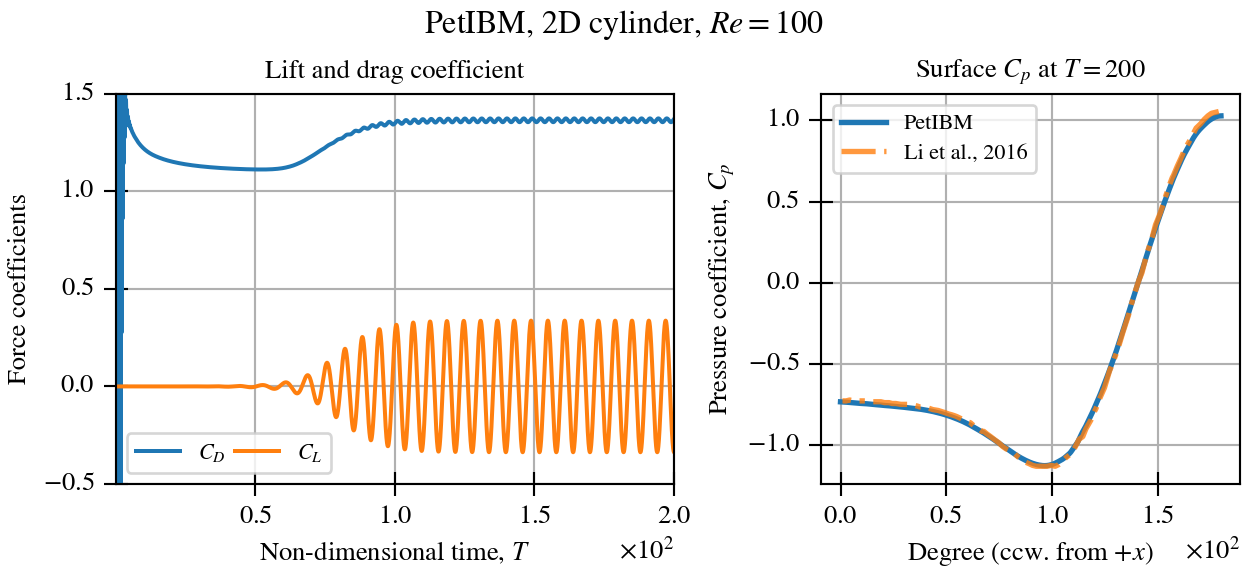
\includegraphics[width=0.95\linewidth]{cylinder-2d-re100/petibm-cylinder-2d-re100-val}
    \caption{PetIBM, 2D cylinder, $Re=100$: drag, lift, and pressure coefficients}
    \label{fig:petibm-cylinder-2d-re100-val}
\end{figure}
The drag coefficient and Strouhal number were verified with others' published numerical data and shown in table \ref{table:cylinder-2d-re100-comparison-cd}.
Figure \ref{fig:petibm-cylinder-2d-re100-val} shows the drag and lift coefficient with respect to time and the distribution of surface pressure coefficients.
The latter was verified against another published simulation result.

We determined that the V\&V for 2D cylinder flow at $Re=100$ was successful.

\subsection*{Validation of 3D flow around a sphere}

We validate the simulation results of 3D sphere flows at different Reynolds numbers.
These Reynolds numbers are $Re=50, 100, 150, 200, 250, 300$.
All cases used the same computational domain, $[-10, 10] \times [-10, 10] \times [-10, 10]$, and the time step size $\Delta t=0.004$.
The corresponding grid sizes are $272 \times 82 \times 82$.
The BCs, ICs, and the linear solver configurations are the same as those in 2D cylinder flow at $Re=100$.

Figure \ref{fig:petibm-sphere3d-drag-val} shows the validation results against experimental data \cite{clift_bubbles_2013,roos_experimental_1971}.
\begin{figure}[hbt!]
    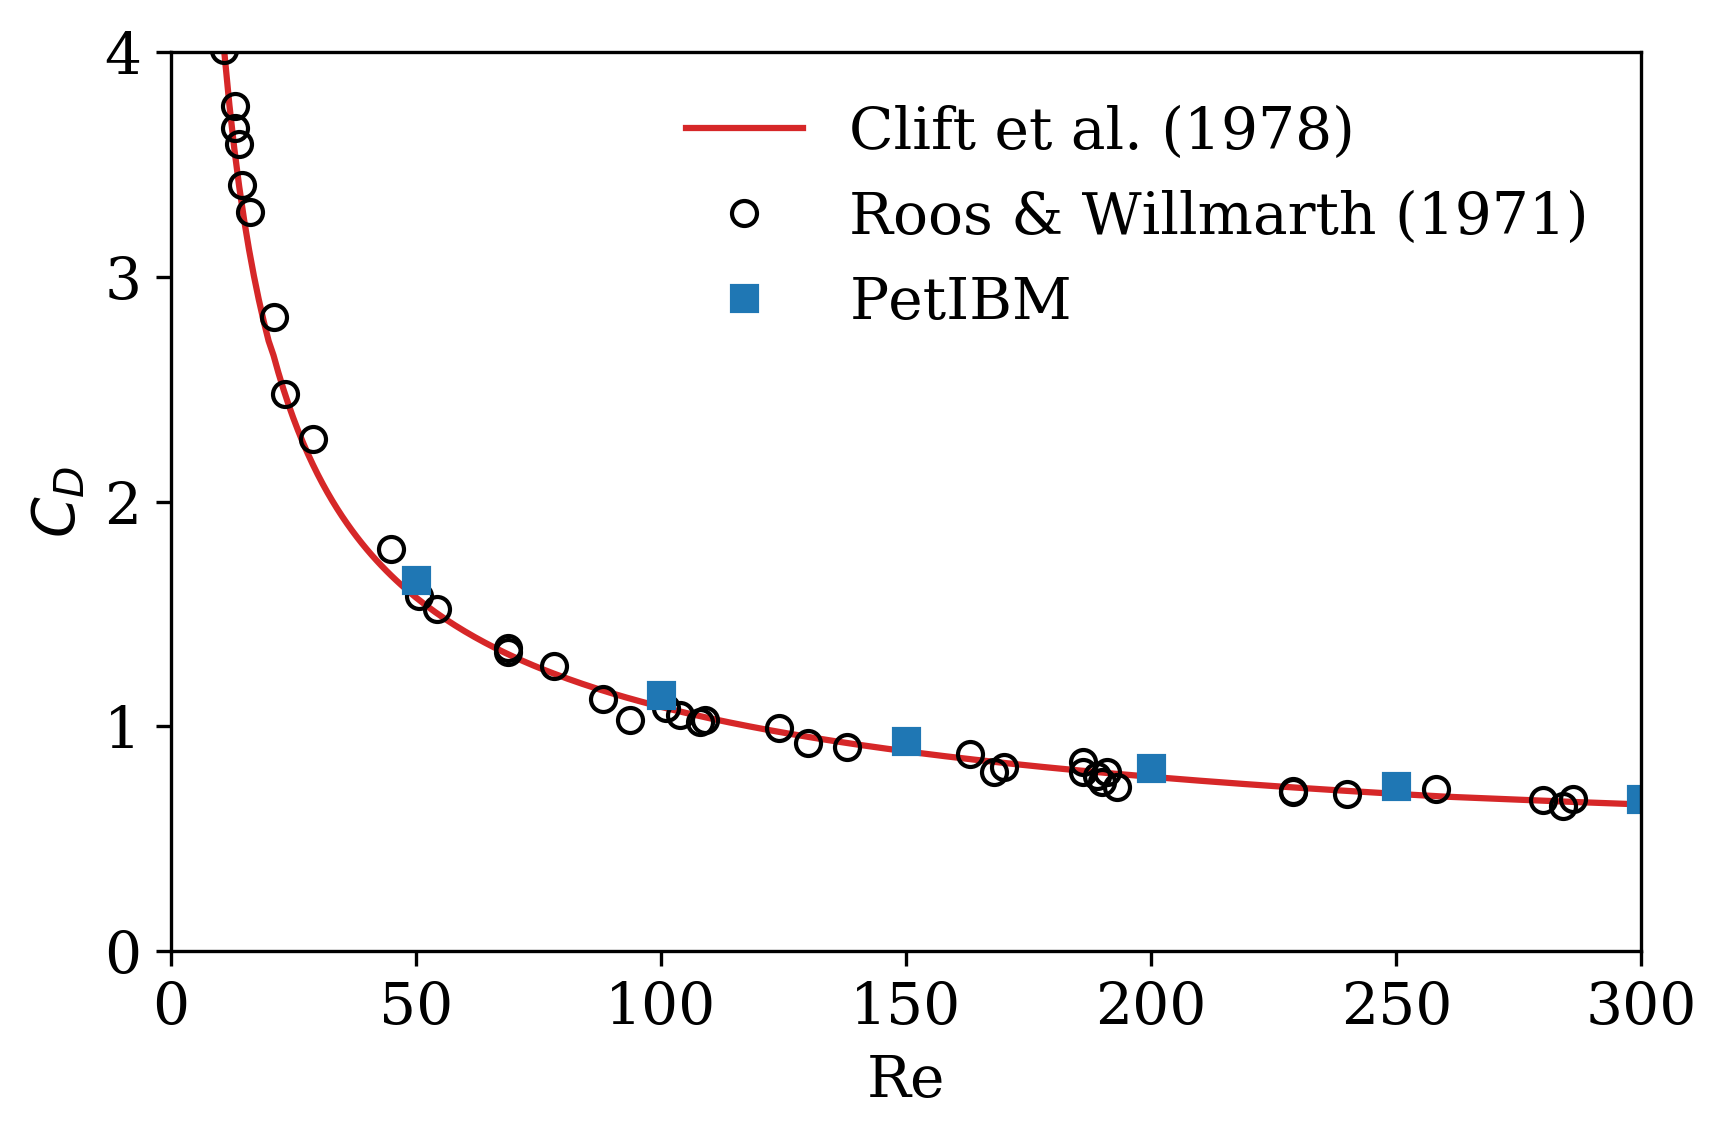
\includegraphics[width=0.6\linewidth]{sphere-3d/drag_coefficient}
    \caption[PetIBM, 3D sphere: drag coefficient validation]{
        PetIBM, 3D sphere: drag coefficient validation \cite{clift_bubbles_2013,roos_experimental_1971}
    }
    \label{fig:petibm-sphere3d-drag-val}
\end{figure}
We believe it is proper to call the validation of 3D sphere flow a success.

\subsection*{Validation of 3D flow around an inclined flat plate}

Lastly, we validate the solver using a 3D flow over an inclined flat plate at $Re=100$.
We tested with several AoA (angle of attack) and validated the results against the experimental data from \cite{taira_unsteadiness_2007}.
All cases had the same computational domain, $[-4, 6.1] \times [-5, 5] \times [-5, 5]$.
And the flat plate was located at $(0.1, 1, 1)$.
The spatial discretization is $192 \times 56 \times 86$, and the time step $\Delta t$ is $0.01$.
The BCs, ICs, and the linear solver configurations are the same as those in 2D cylinder flow at $Re=100$.

\begin{figure}[hbt!]
    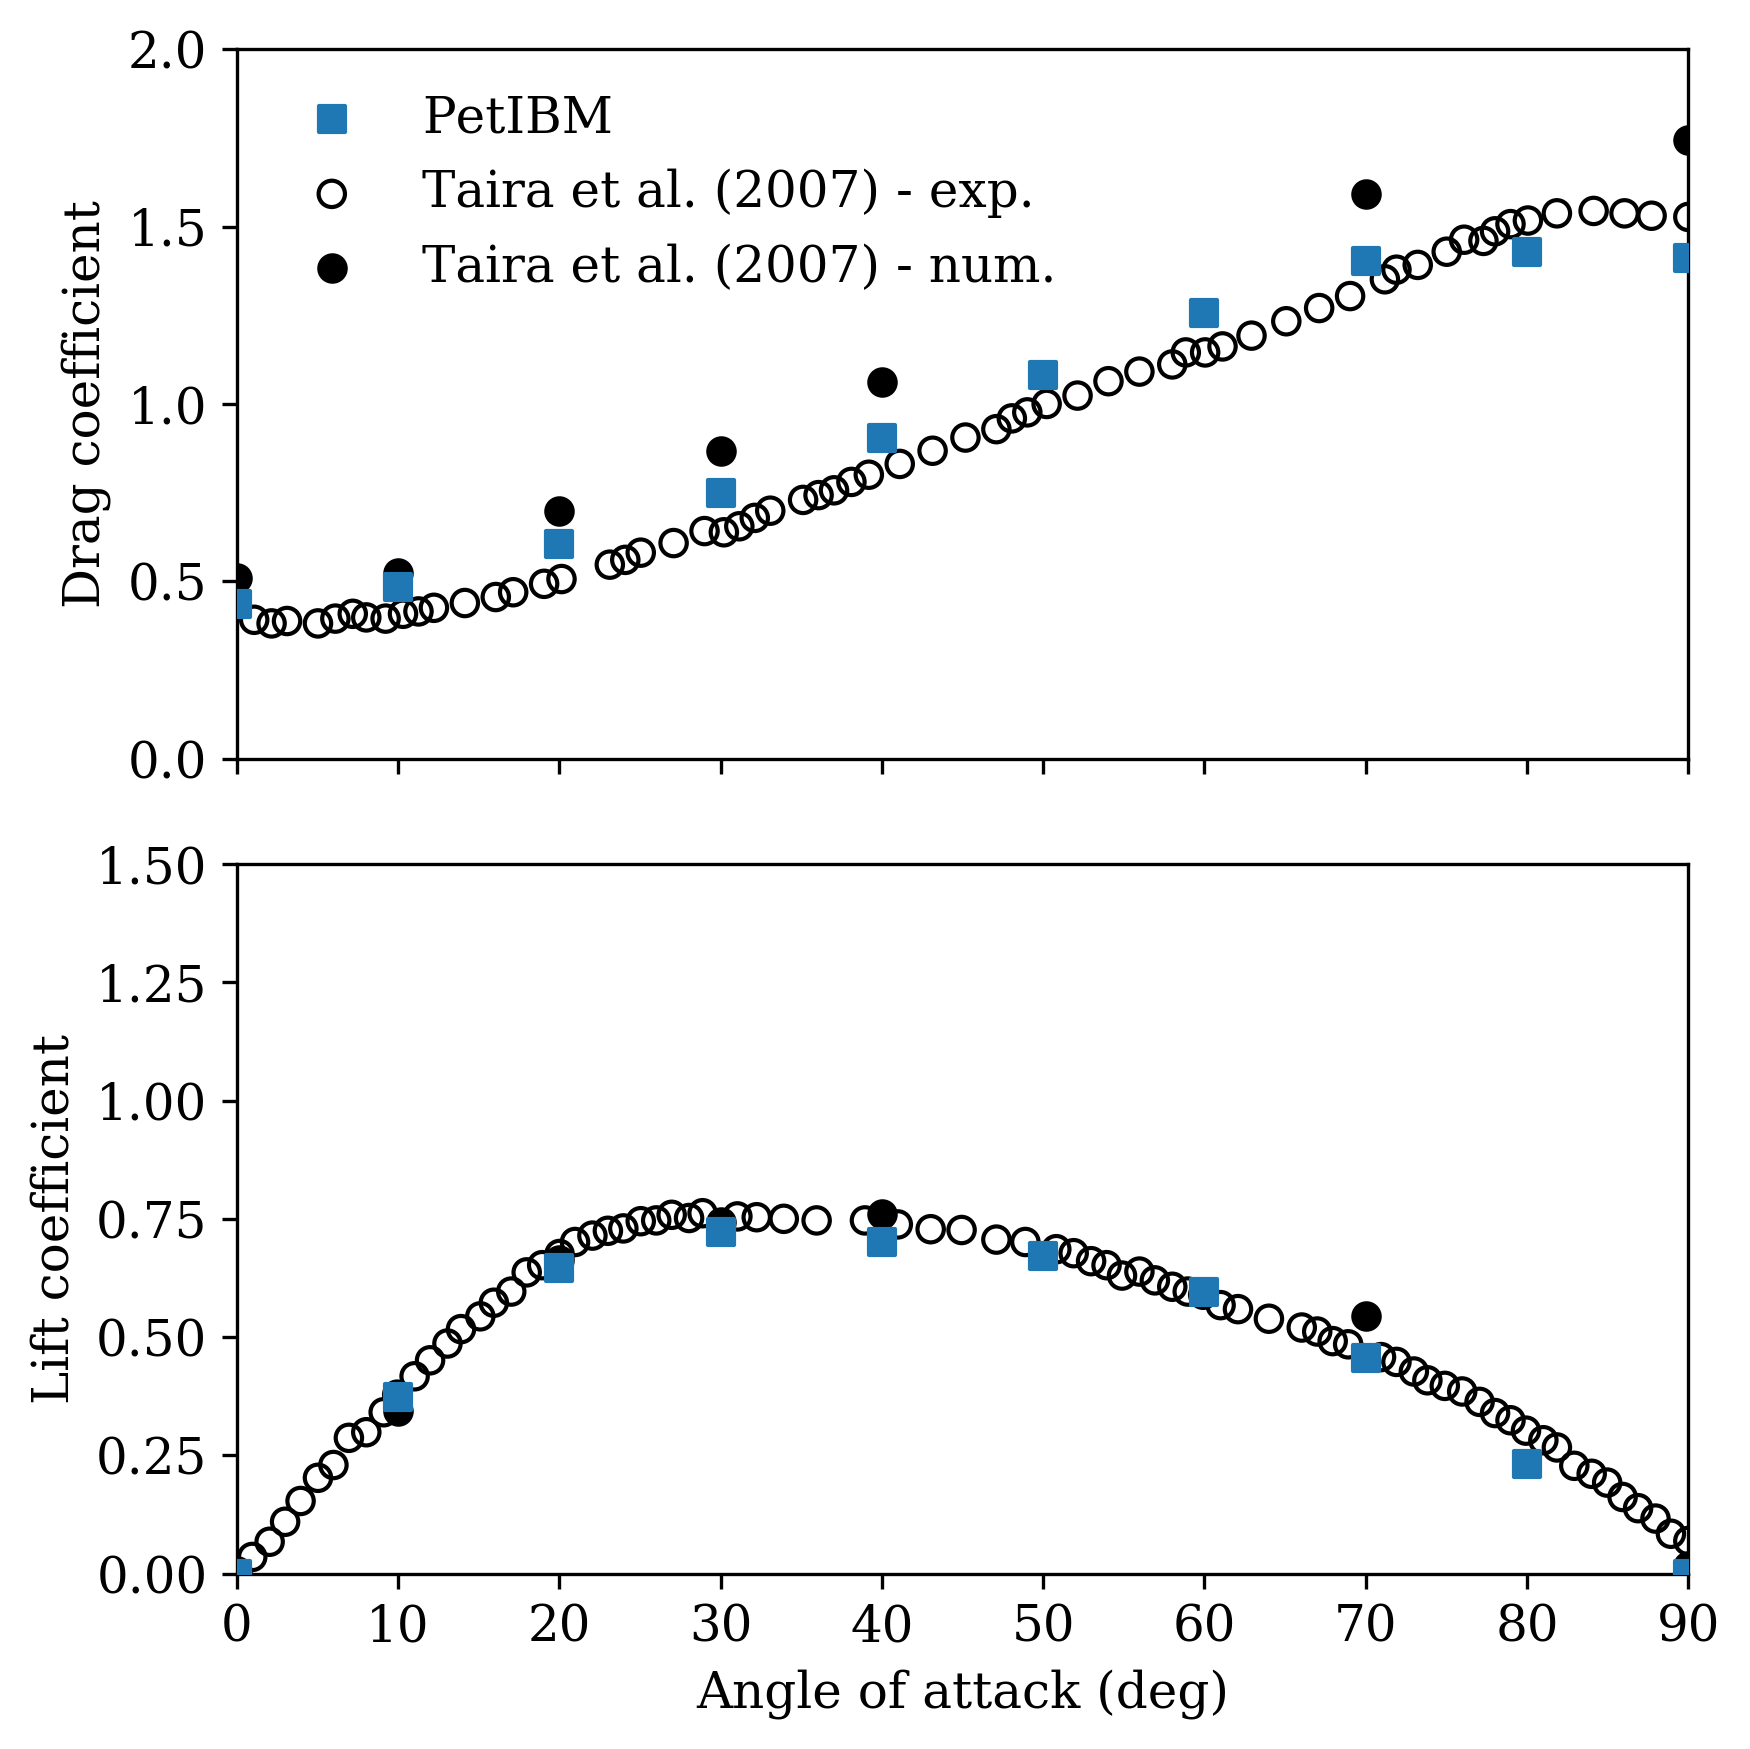
\includegraphics[width=0.6\linewidth]{plate-3d-re100/force_coefficients}
    \caption{PetIBM, 3D plate: drag and lift coefficient validation}
    \label{fig:petibm-plate3d-drag-lift-val}
\end{figure}
Figure \ref{fig:petibm-plate3d-drag-lift-val} shows that the experimental data matches our numerical simulation well.

% vim:ft=tex